%!TEX program = xelatex
\documentclass{lni}

\IfFileExists{latin1.sty}{\usepackage{latin1}}{\usepackage{isolatin1}}

\usepackage{graphicx}
\usepackage{fancyhdr}
\usepackage{listings} %if lstlistings is used
\usepackage{changepage} %for changing topmargin on first page
\usepackage[figurename=Abb., tablename=Tab., small]{caption}[2008/04/01]
\renewcommand{\lstlistingname}{List.}    % Listingname heit nun List. 
\usepackage{fontspec}
\usepackage{todonotes}
\usepackage{float}

%Beginn der Seitenzählung für diesen Beitrag
\setcounter{page}{1}

%Kopfzeileneinstellungen
\pagestyle{fancy}
\fancyhead{} % Lscht alle Kopfzeileneinstellungen
%\fancyhead[RO]{\small $<$Christian Blank [et. al.]$>$(Hrsg.): $<$Buchtitel$>$, \linebreak Lecture Notes in Informatics (LNI), Gesellschaft fr Informatik, Bonn $<$Jahr$>$ \hspace{5pt} \thepage \hspace{0.05cm}}
%\fancyfoot{} % Lscht alle Fuzeileneinstellungen
\renewcommand{\headrulewidth}{0.4pt} %Linie unter Kopfzeile 
\setcounter{footnote}{0}

\author{Iwer Petersen - $I^2E$ Interactive Immersive Environments}
\title{Projekt2 - Online User Rekonstruktion}
\begin{document}
\maketitle
%Überschrift des Literaturverzeichnisses
\renewcommand{\refname}{Literaturverzeichnis}
\setcounter{footnote}{1} %Auf Anzahl der AutorInnen setzen, damit die weitere Nummerierung der Funoten passt

%


%!TEX root = paper.tex
\begin{abstract}

\end{abstract}
\begin{keywords}
\end{keywords}
%!TEX root = ../paper.tex
\section{Einführung}
\label{sec:user_reconstruction}

% Einsatz von Spielmechaniken in verschiedenen organisationalen Kontexten (z.B. Wissensmanagement, Innovationsmanagement, Aus- und Weiterbildung)
% Anwendung virtueller Welten in der Unternehmenskommunikation und -kollaboration
% Einsatz virtueller Welten im Innovationsprozess und in der Kundenintegration
% Integration der Technologie virtueller Welten mit anderen Technologien und Informationssystemen

In verteilten, kollaborativen Multi-User MR-Umgebungen sind konfliktträchtige 
Handlungen zwischen Usern immanent. Abhilfe schafft hier eine realistische 
virtuelle Darstellung entfernter User innerhalb der virtuellen Szene, so dass 
sie von anderen Teilnehmer mittels VR-See-Through-Brillen wahrgenommen werden 
kann. So können Konflikte schon durch Erkennen der Intentionen entfernter User 
vermieden werden. Dieser Ansatz, der von \cite{Cassell:2000:ECI:332051.332075} 
beschrieben wurde, wird unter anderem in den Arbeiten von \cite{mcmanus2011influence} und \cite{dodds2011talk} verifiziert, die mit Hilfe von selbst-animierten Avataren 
- welche durch Motion-Capturing die Bewegungen von Benutzern abbilden - 
nachgewiesen haben, dass dieses Vorgehen die Kommunikation zwischen Usern sowie 
die Koordination von Handlungen in virtuellen, kollaborativen Umgebungen 
verbessert.

\begin{figure}[H]
	\centering
	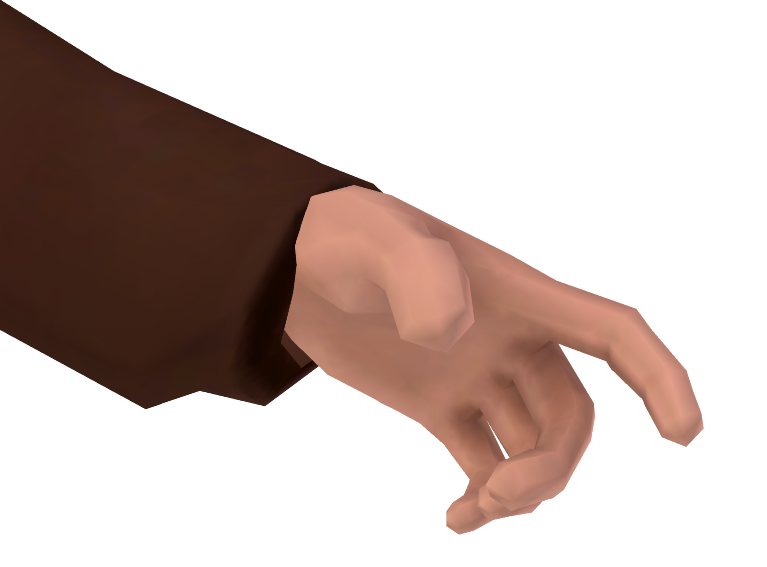
\includegraphics[width=.3\textwidth]{figs/anim-ok}
	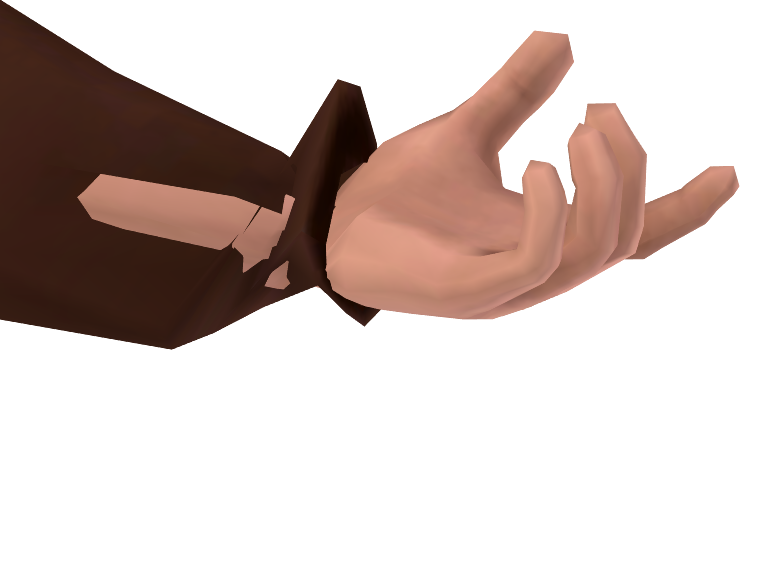
\includegraphics[width=.3\textwidth]{figs/anim-prob}
	\caption{Unrealistische Verformung eines statischen Charaktermodells bei 
	starker Handdrehung}
	\label{fig:animationproblem}
\end{figure}

Die Probleme die üblicherweise bei Charakteranimation auftreten (siehe Abbildung 
\ref{fig:animationproblem}) sowie Ungenauigkeiten beim Motion-Capturing lassen 
allerdings keine beliebig hohe Detaillierung des Avatars zu. Weiterhin kann die 
Komplexität des Skelettmodells schnell sehr groß werden, wenn zum Beispiel 
Details wie Gesichtsausdrücke abgebildet werden sollen. Eine Alternative zur 
Charakteranimation stellt ein Echtzeit-Rekonstruktionsverfahren dar, welches 
3D Modelle der User mittels 3D Sensoren erzeugt. Durch die Markteinführung der 
Microsoft Kinect Kamera sind solche Sensoren deutlich erschwinglicher geworden, 
was zu einer Reihe von wissenschaftlichen Arbeiten geführt hat, die weitere 
Einsatzgebiete des Sensors betrachten. Die Erfassung von statischen 3D Modellen 
mit Hilfe von Kinect Kameras wurde auf Basis von Punktwolken 
(siehe \cite{tong2012scanning}) sowie Distanzfunktionen 
\cite{Izadi:2011:KRR:2047196.2047270} realisiert und die prinzipielle Eignung 
der Kinect als Sensor für 3D Rekonstruktion gezeigt. Im Gegensatz zur 
Rekonstruktion statischer Modelle stehen einer Echtzeit-Rekonstruktion 
lediglich einzelne Frames zur Verfügung, die in drastisch reduzierter Zeit 
verarbeitet werden müssen. Erste Versuche einer Echtzeitrekonstruktion für 
tele-immersive Anwendungen wurden bereits von \cite{alexiadis2013real} gemacht 
und mit Hilfe von \cite{mekuria2013teleimmersion} zu einer funktionierenden 
Streaming Pipeline ausgebaut. Dank ausgeklügelten Kompressionsstrategie erreicht 
das System auf dem darstellenden Zielsystem eine Framerate von 5 - 8 Bildern 
pro Sekunde.

\section{Konzept}
% Pipeline wie Me13, Optimierung durch Downsampling, Einzelbildrekonstruktion
Im Gegensatz zu der Methode von \cite{alexiadis2013real}, welche zunächst 
Teilmeshes aus den Daten der einzelnen Kameras generiert und diese dann 
vereinigt, sollen hier zunächst die Punktwolken der einzelnen Kameras vereinigt 
werden und anschließend trianguliert werden. Das Ziel ist hierbei, ein 3D Modell 
mit geringerer Datenmenge zu erhalten, welches performanter gestreamt werden 
kann. Die Datenmenge in einem 3D Modell wird durch die Anzahl der Vertizen sowie 
Anzahl an Verbindungen zwischen Vertizen bestimmt. Essentiell ist das Ziel also 
ein 3D Modell mit einer geringeren Vertizen Anzahl zu erhalten, welches trotz 
geringerer Datenmenge eine ausreichende visuelle Qualität behält. Um das bei 
einer niedrigeren Punktauflösung sicherstellen zu können, sollen Punkte keine 
Farbe sondern Texturkoordinaten erhalten welche ein 3D Texturmapping ermöglichen.


\begin{figure}[H]
	\centering
	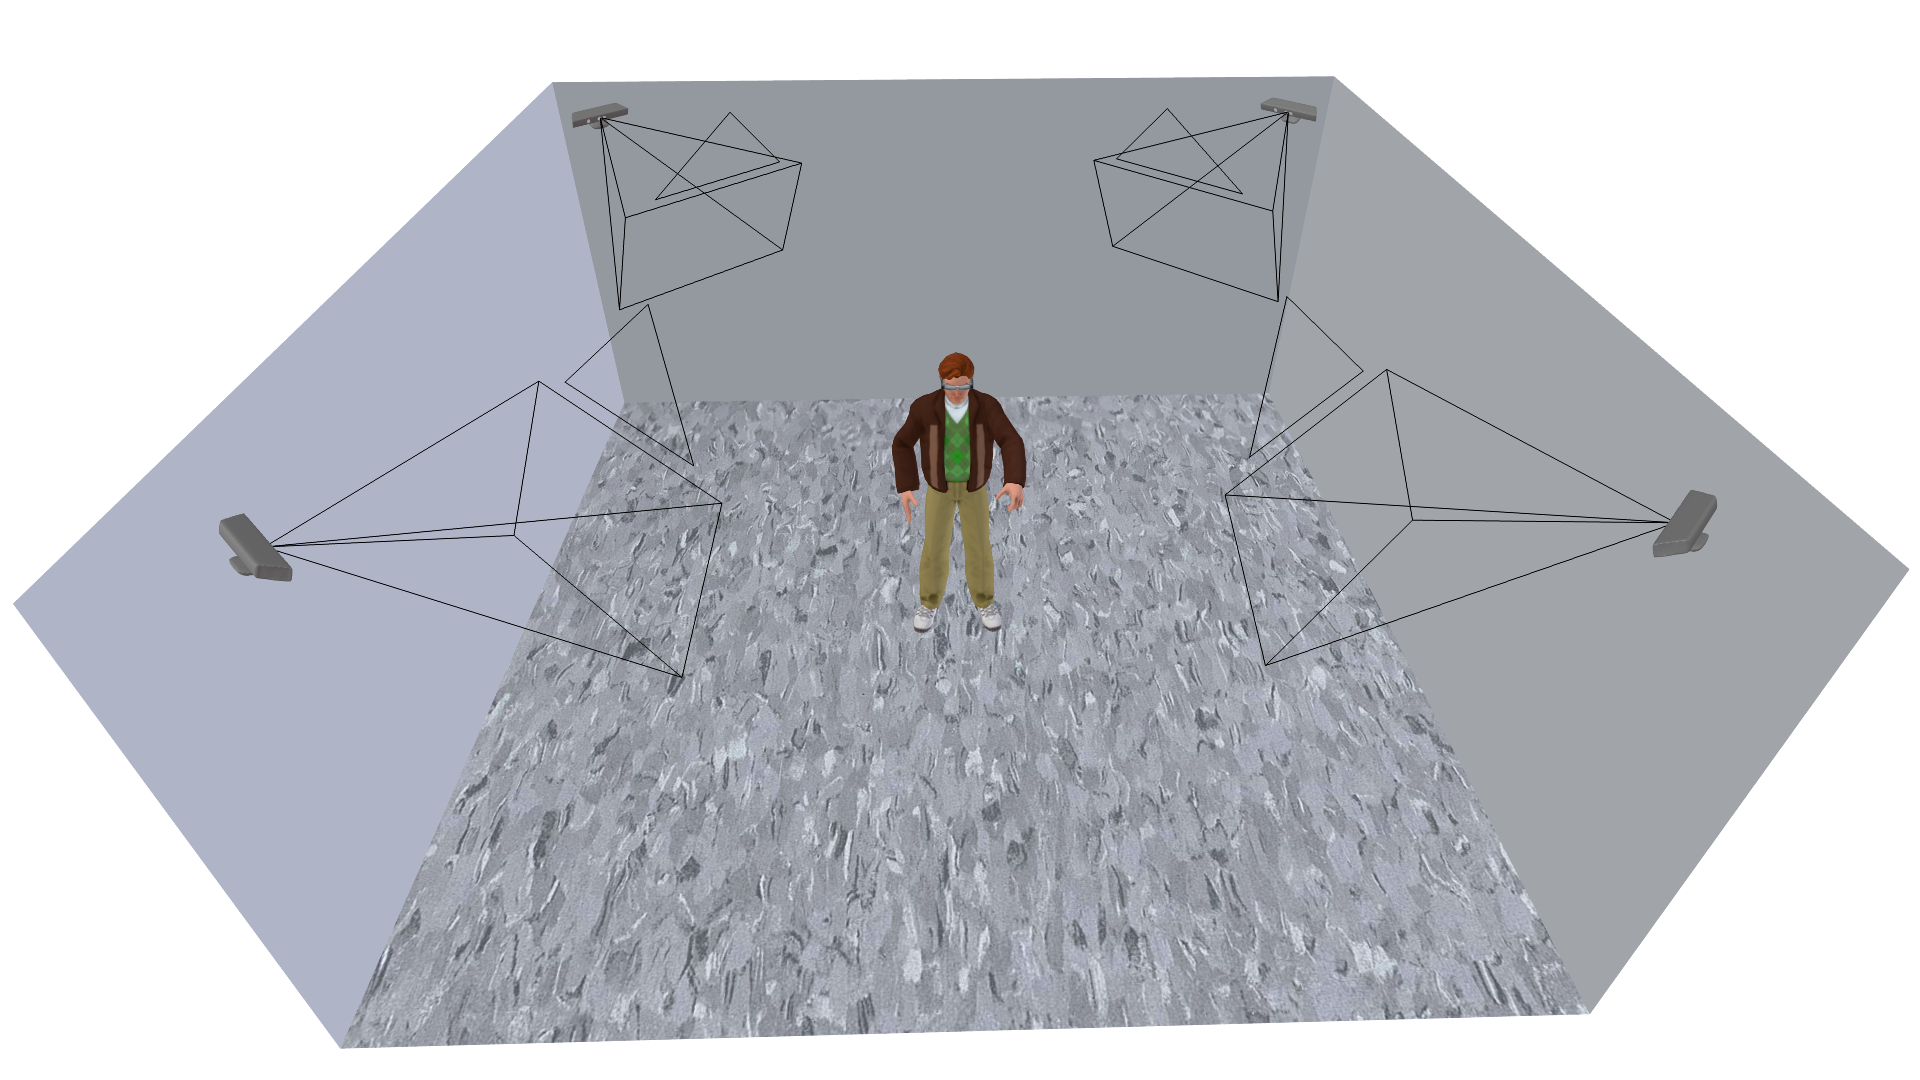
\includegraphics[width=.7\textwidth]{figs/scanning_setup}
	\caption{Versuchsaufbau des Scansystems um eine zu rekonstruierende Person}
	\label{fig:recon_setup}
\end{figure}

Um 3D Modelle von Usern des MR-Systems auf einer entfernten System-Instanz 
darstellen zu können, müssen diese zunächst durch eine Echtzeit Scanning 
Komponente erfasst und anschließend über eine Netzwerkverbindung an ein 
darstellendes System versendet werden. Ähnlich wie das System von 
\cite{alexiadis2013real} und \cite{mekuria2013teleimmersion} werden Microsoft 
Kinect Kameras als Sensoren verwendet, um aus den Tiefenbildern 3D Informationen 
der Umgebung zu erhalten. Dazu werden um einen definierten Bereich die Kameras 
so installiert, dass sie eine möglichst hohe Abdeckung der Personen innerhalb 
des Scanbereichs erreichen (siehe Abbildung \ref{fig:recon_setup}). Um eine 
gemeinsame räumliche Ausrichtung der Kameradaten zu ermöglichen sind 
extrinsische sowie intrinsische Parameter der Kameras mit Hilfe einer 
Kalibrierungsmethode zu erfassen.

\subsection{Rekonstruktions-Pipeline}

% Offline Kalibrierung, Reko-Pipeline, Streaming-Komponente

\begin{figure}[H]
	\centering
	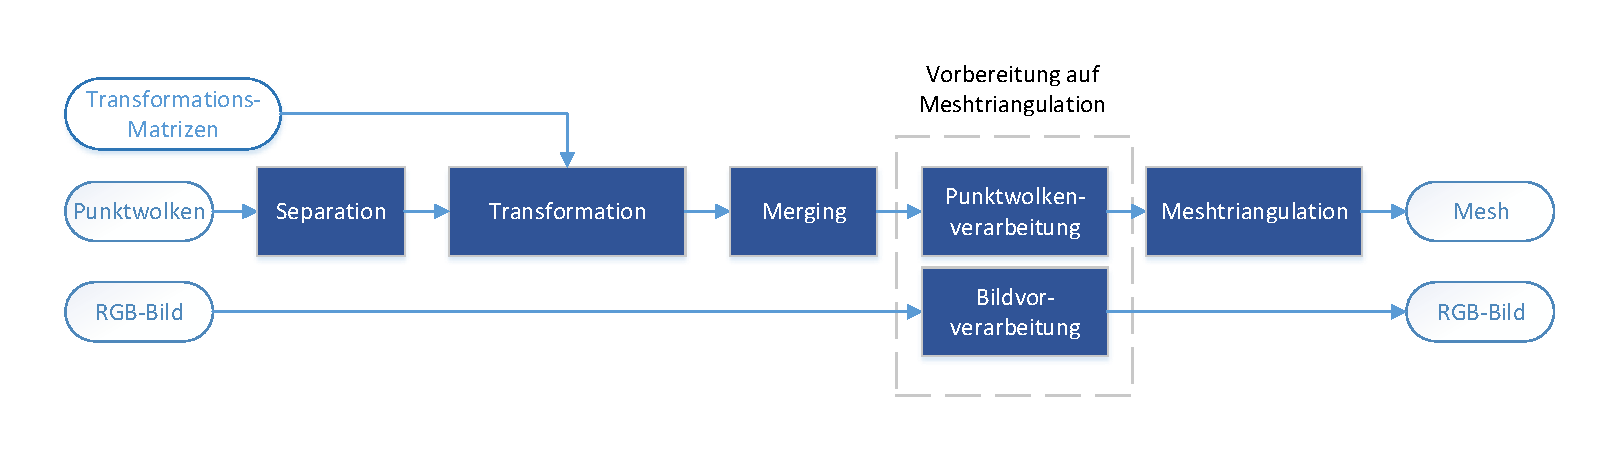
\includegraphics[width=\textwidth]{figs/recon_pipeline}
	\caption{Rekonstruktions-Pipeline}
	\label{fig:recon_pipeline}
\end{figure}

Die von den Kinectkameras generierten Tiefenbildframes werden in einer Pipeline 
in mehreren Schritten zu einem geschlossenen Mesh verarbeitet. Dabei werden die
Farbbilder der Kameras für eine spätere Texturierung mitverarbeitet. Wie in 
Abbildung \ref{fig:recon_pipeline} dargestellt, nimmt die Pipeline aus den 
Tiefenbildern generierten Punktwolken sowie die Farbbilder der Kameras entgegen.
Zunächst wird über eine Hintergrundseparation die zu rekonstruierenden Teile der 
einzelnen Punktwolken freigestellt. Diese besteht momentan aus einem Tiefenthreshold, 
mit dem Punkte, die zu nah oder zu weit weg von der Kamera sind herausgefiltert. In 
Zukunft ist hier zusätzlich der Einsatz einer statischen Hintergrundsubtraktion 
geplant, welche Punkte entfernt, die sehr nah an Punkten eines gespeicherten 
Hintergrundabbildes ist. Mit Hilfe der über eine geeignete 
Kalibrierungsmethode bezogenen Transformationsmatrizen werden die Punktwolken 
dann in ein gemeinsames Koordinatensystem transformiert. Nach der Vereinigung 
der so zueinander ausgerichteten Punktwolken wird die vereinigte Punktwolke auf 
den Meshtriangulationschritt vorbereitet. Der wichtigste Schritt in dieser 
Vorbereitung ist die Reduzierung der Punktanzahl durch Reduzierung der räumlichen 
Auflösung. Weitere Vorbereitungsschritte sind Voraussetzung für eine erfolgreiche 
Triangulation und bestehen aus der Generierung von Oberflächennormalen sowie aus 
einem Glättungsschritt (siehe Abbildung \ref{fig:recon_pipeline_tri}). Anschließend wird 
die Punktwolke mit einem geeigneten Meshtriangulationsverfahren mit einem Gitter 
überzogen.

\begin{figure}[H]
	\centering
	
\includegraphics[width=\textwidth]{figs/tri_pipe}
	\caption{Rekonstruktions-Pipeline: Detailansicht Mesh-Triangulation}
	\label{fig:recon_pipeline_tri}
\end{figure}

Die Farbbilder der einzelnen Kameras werden zunächst in einer Matrix zu einem 
einzelnen Bild angeordnet. Durch Rücktranformation der Punkte in die 
Kameraebenen der RGB-Kameras werden für jeden Punkt Texturkoordinaten auf der 
vereinigten Textur erzeugt. Dies ermöglicht ein späteres Mapping der Textur auf 
des 3D Modell.

Das rekonstruierte Mesh sowie die vereingte Textur bilden nun die Grundlage für 
ein 3D Modell für eine Visualisierung in einer 3D Umgebung. Da das Modell unter 
Umständen auch an einem entfernten Ort visualisiert werden soll wird das 3D 
Modell über eine Netzwerkschnittstelle an das Zielsystem versendet. Hierbei wird 
zunächst auf die Projekt-Middleware gesetzt. Da der verfolgte Rekonstruktionsansatz 
primär auf die Datenreduktion zielt, wird zunächst auf eine weitere Kompression verzichtet.

\subsubsection{Aktueller Stand: }
\begin{figure}[H]
	\centering
	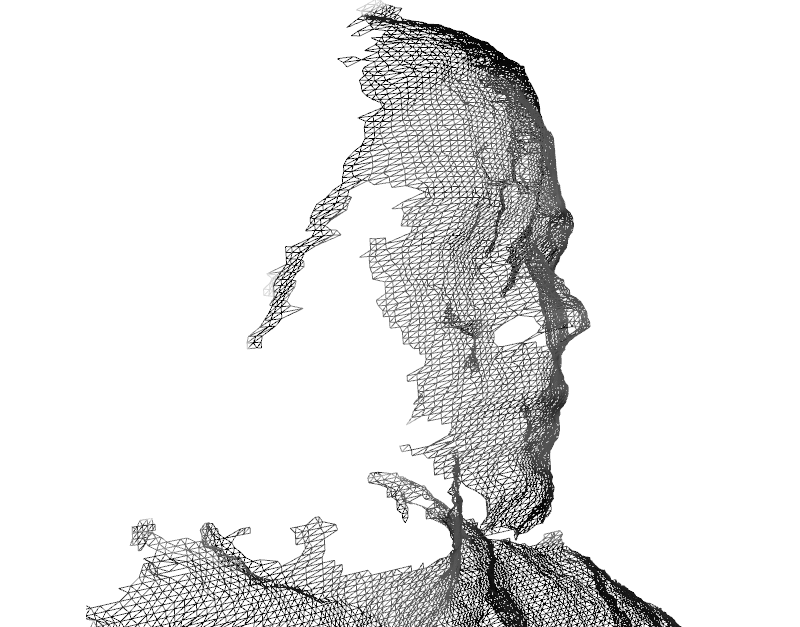
\includegraphics[width=.5\textwidth]{figs/recon_wireframe}
	\caption{2,5D Triangulation einer einzelnen Kamera}
	\label{fig:2dmeshed}
\end{figure}

Erste Experimente mit der Rekonstruktion aus von der 
Kinect generierten Punktwolken wurden mit einer einzelnen Kamera gemacht. Mit 
einem 2,5D Triangulationsalgorithmus, der die bekannte Nachbarschaft der Pixel 
eines Tiefenbildes ausnutzt um benachbarte 3D Punkte zu verbinden, können Halbschalen 
eines 3D Modells sehr schnell erzeugt werden. Je nach räumlicher Auflösung der 
Punkte sind 10 - 60 Rekonstruktionen pro Sekunde erreichbar. Der verwendete 
Algorithmus ist dem von \cite{alexiadis2013real} verwendetem Algorithmus sehr 
ähnlich, erfordert bei der Verwendung mehrerer Kameras aber die aufwändige 
Vereinigung der einzelnen Meshes. Da die Information über Punktnachbarschaften 
bei der Vereinigung der Punktwolken mehrerer Kameras nicht erhalten bleibt, ist 
die Anwendung eines 2,5D Triangulationsalsgorithmus bei einer solchen vereinigten 
Punktwolke erst einmal nicht möglich.

\begin{figure}[H]
	\centering
	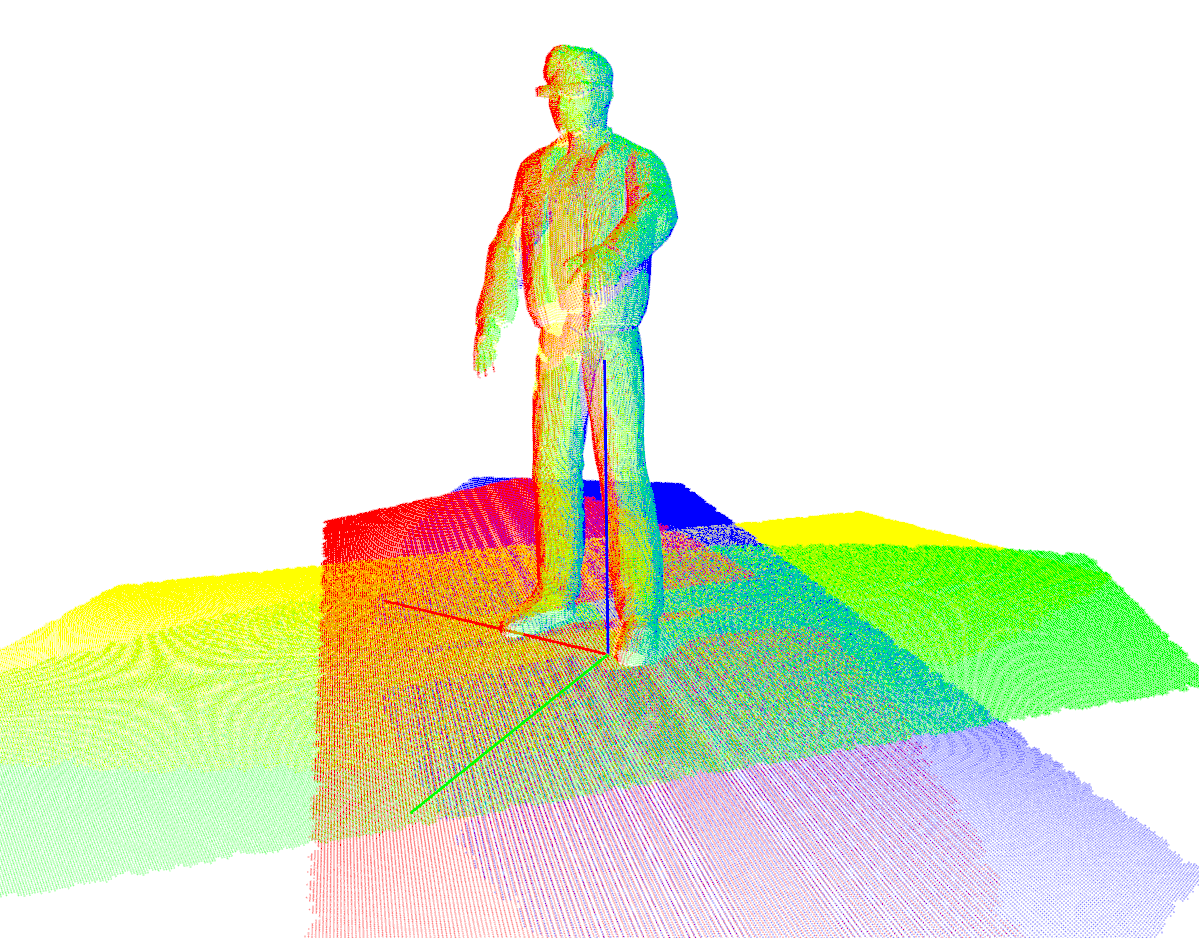
\includegraphics[width=.5\textwidth]{figs/registered_pointclouds}
	\caption{In Weltkoordinaten transformierte Punktwolken von vier 
		Kinectkameras (rot, blau, grün, gelb). Die Punktwolken wurden mit 
		Blensor \cite{Gschwandtner11b} aus der Szene in Abbildung 
		\ref{fig:recon_setup} generiert.}
	\label{fig:cloud_sources}
\end{figure}

Zum Entwickeln der Rekonstruktionspipeline werden simulierte Sensordaten 
verwendet, welche mit der Sensorsimulations-Software Blensor 
(siehe \cite{Gschwandtner11b}) erstellt werden. Dadurch können beliebige 
Szenarien als 3D Modell erstellt und resultierende Sensordaten ohne aufwändige 
Kalibrierung gewonnen werden, da die Positionen der Kameras wohlbekannt sind. 
Für einen späteren Real-Life Einsatz ist natürlich die Implementierung eines 
komfortablen Multikamera-Kalibrierungsverfahrens notwendig. Ein 
vielversprechender Kandidat ist das Verfahren von Staranowicz et. al. 
\cite{staranowicz2014easy}, welches mit einem kugelförmigen Kalibrierungsobjekt 
die Kalibrierungsparameter mehrerer Kameras simultan bestimmt.

\begin{figure}[H]
	\centering
	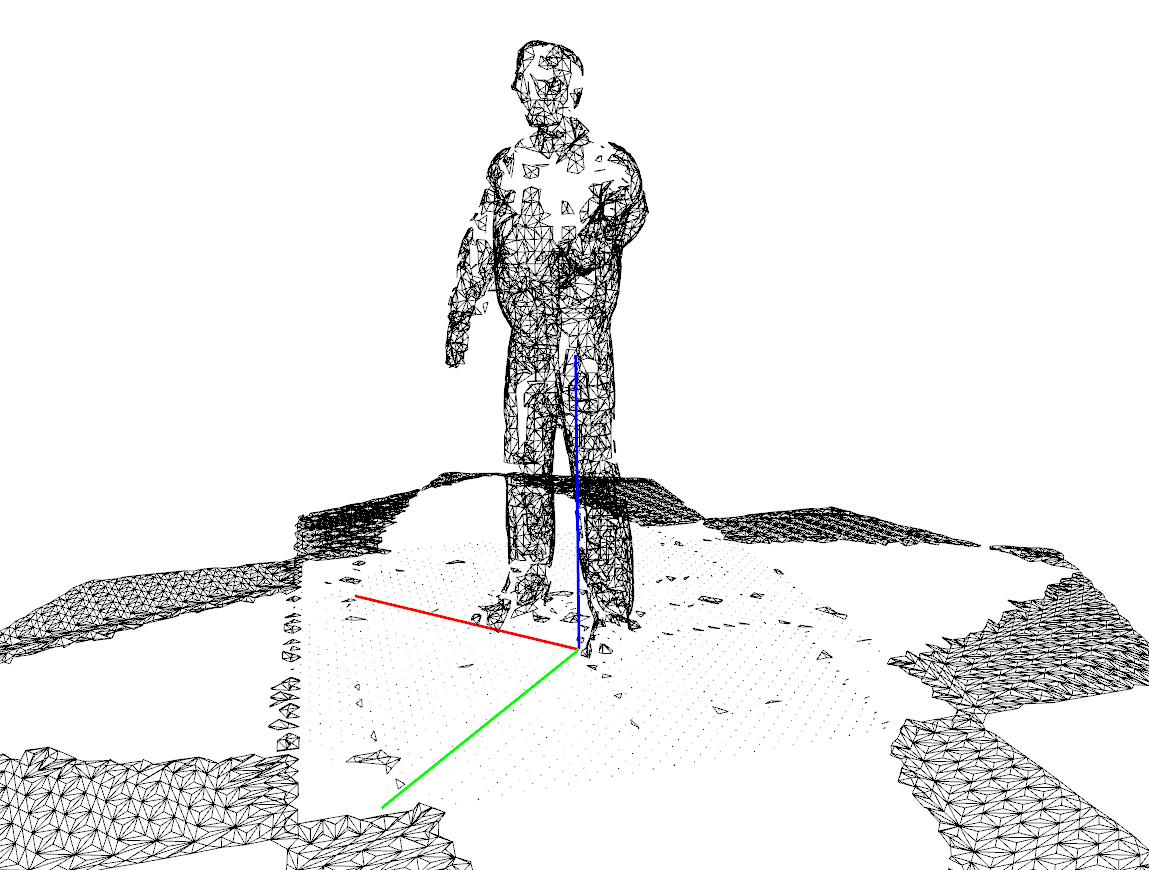
\includegraphics[width=.5\textwidth]{figs/meshed}
	\caption{3D Triangulation mittels Greedy-Projektion}
	\label{fig:meshed}
\end{figure}

% Ref fig:meshed Greedy Projection Triangulation aktueller Stand
% Fehlt noch Background subtraction, Pointcloud Optimierung (Smoothing)
% Evtl. Rückschritt auf 2,5D Triangulation + Mesh-Zippering

Zur Triangulation der vereinigten Punktwolke wurden die ersten Experimente mit 
einem Greedy-Projection Algorithmus (siehe \cite{Marton09ICRA}) gemacht. Dieser 
Algorithmus nutzt Oberflächennormalen um entlang ihren Richtung eine lokale 
Ebene zu projizieren, in welcher mittels einer KD-Tree Repräsentation der Punktwolke 
nach benachbarten Punkten gesucht wird, welche dann zu einem Mesh verbunden 
werden. Dieser Algorithmus erfordert einigermaßen glatte Oberflächen, was sich 
vor allem über die verwendeten Oberflächennormalen auswirkt. Der naive Versuch, die 
rohe, vereinigte Punktwolke zu triangulieren zeigt deutlich die Nachteile der 
fehlenden Nachbarschaftsverhältnisse. In einer Auflösung, in der einzelne 
Punktwolken mit einem 2,5D Algorithmus bei 25 - 30 Rekonstruktionen pro Sekunde 
verarbeitet werden, benötigt dieser Algorithmus eine Sekunde für eine 
Rekonstruktion. Wie in Abbildung \ref{fig:meshed} sind bei diesem Versuch keine 
Maßnahmen zur Punktreduktion wie zum Beispiel Hintergrundseparierung 
durchgeführt worden. Auch ist die räumliche Auflösung der Punktwolke in diesem 
Beispiel weit höher als es möglicherweise für ein funktionables 3D Modell nötig 
ist.


Um diese Pipeline zu realisieren wurde das in Projekt 1 vorgestellte Konzept um 
abstrakte Sensoren erweitert. Diese beinhalten die eigentlichen 
Punktwolkengeneratoren sowie Methoden um eine Hintergrundpunktwolke sowie 
Kalibrierungsparameter festzulegen. Mit diesem Modell können analog zu reellen 
Kameras simulierte Kameras verwendet werden, die zum Beispiel die Mit Blensor 
generierten Punktwolken an die Pipeline auszuliefern.

\begin{figure}[H]
	\centering
	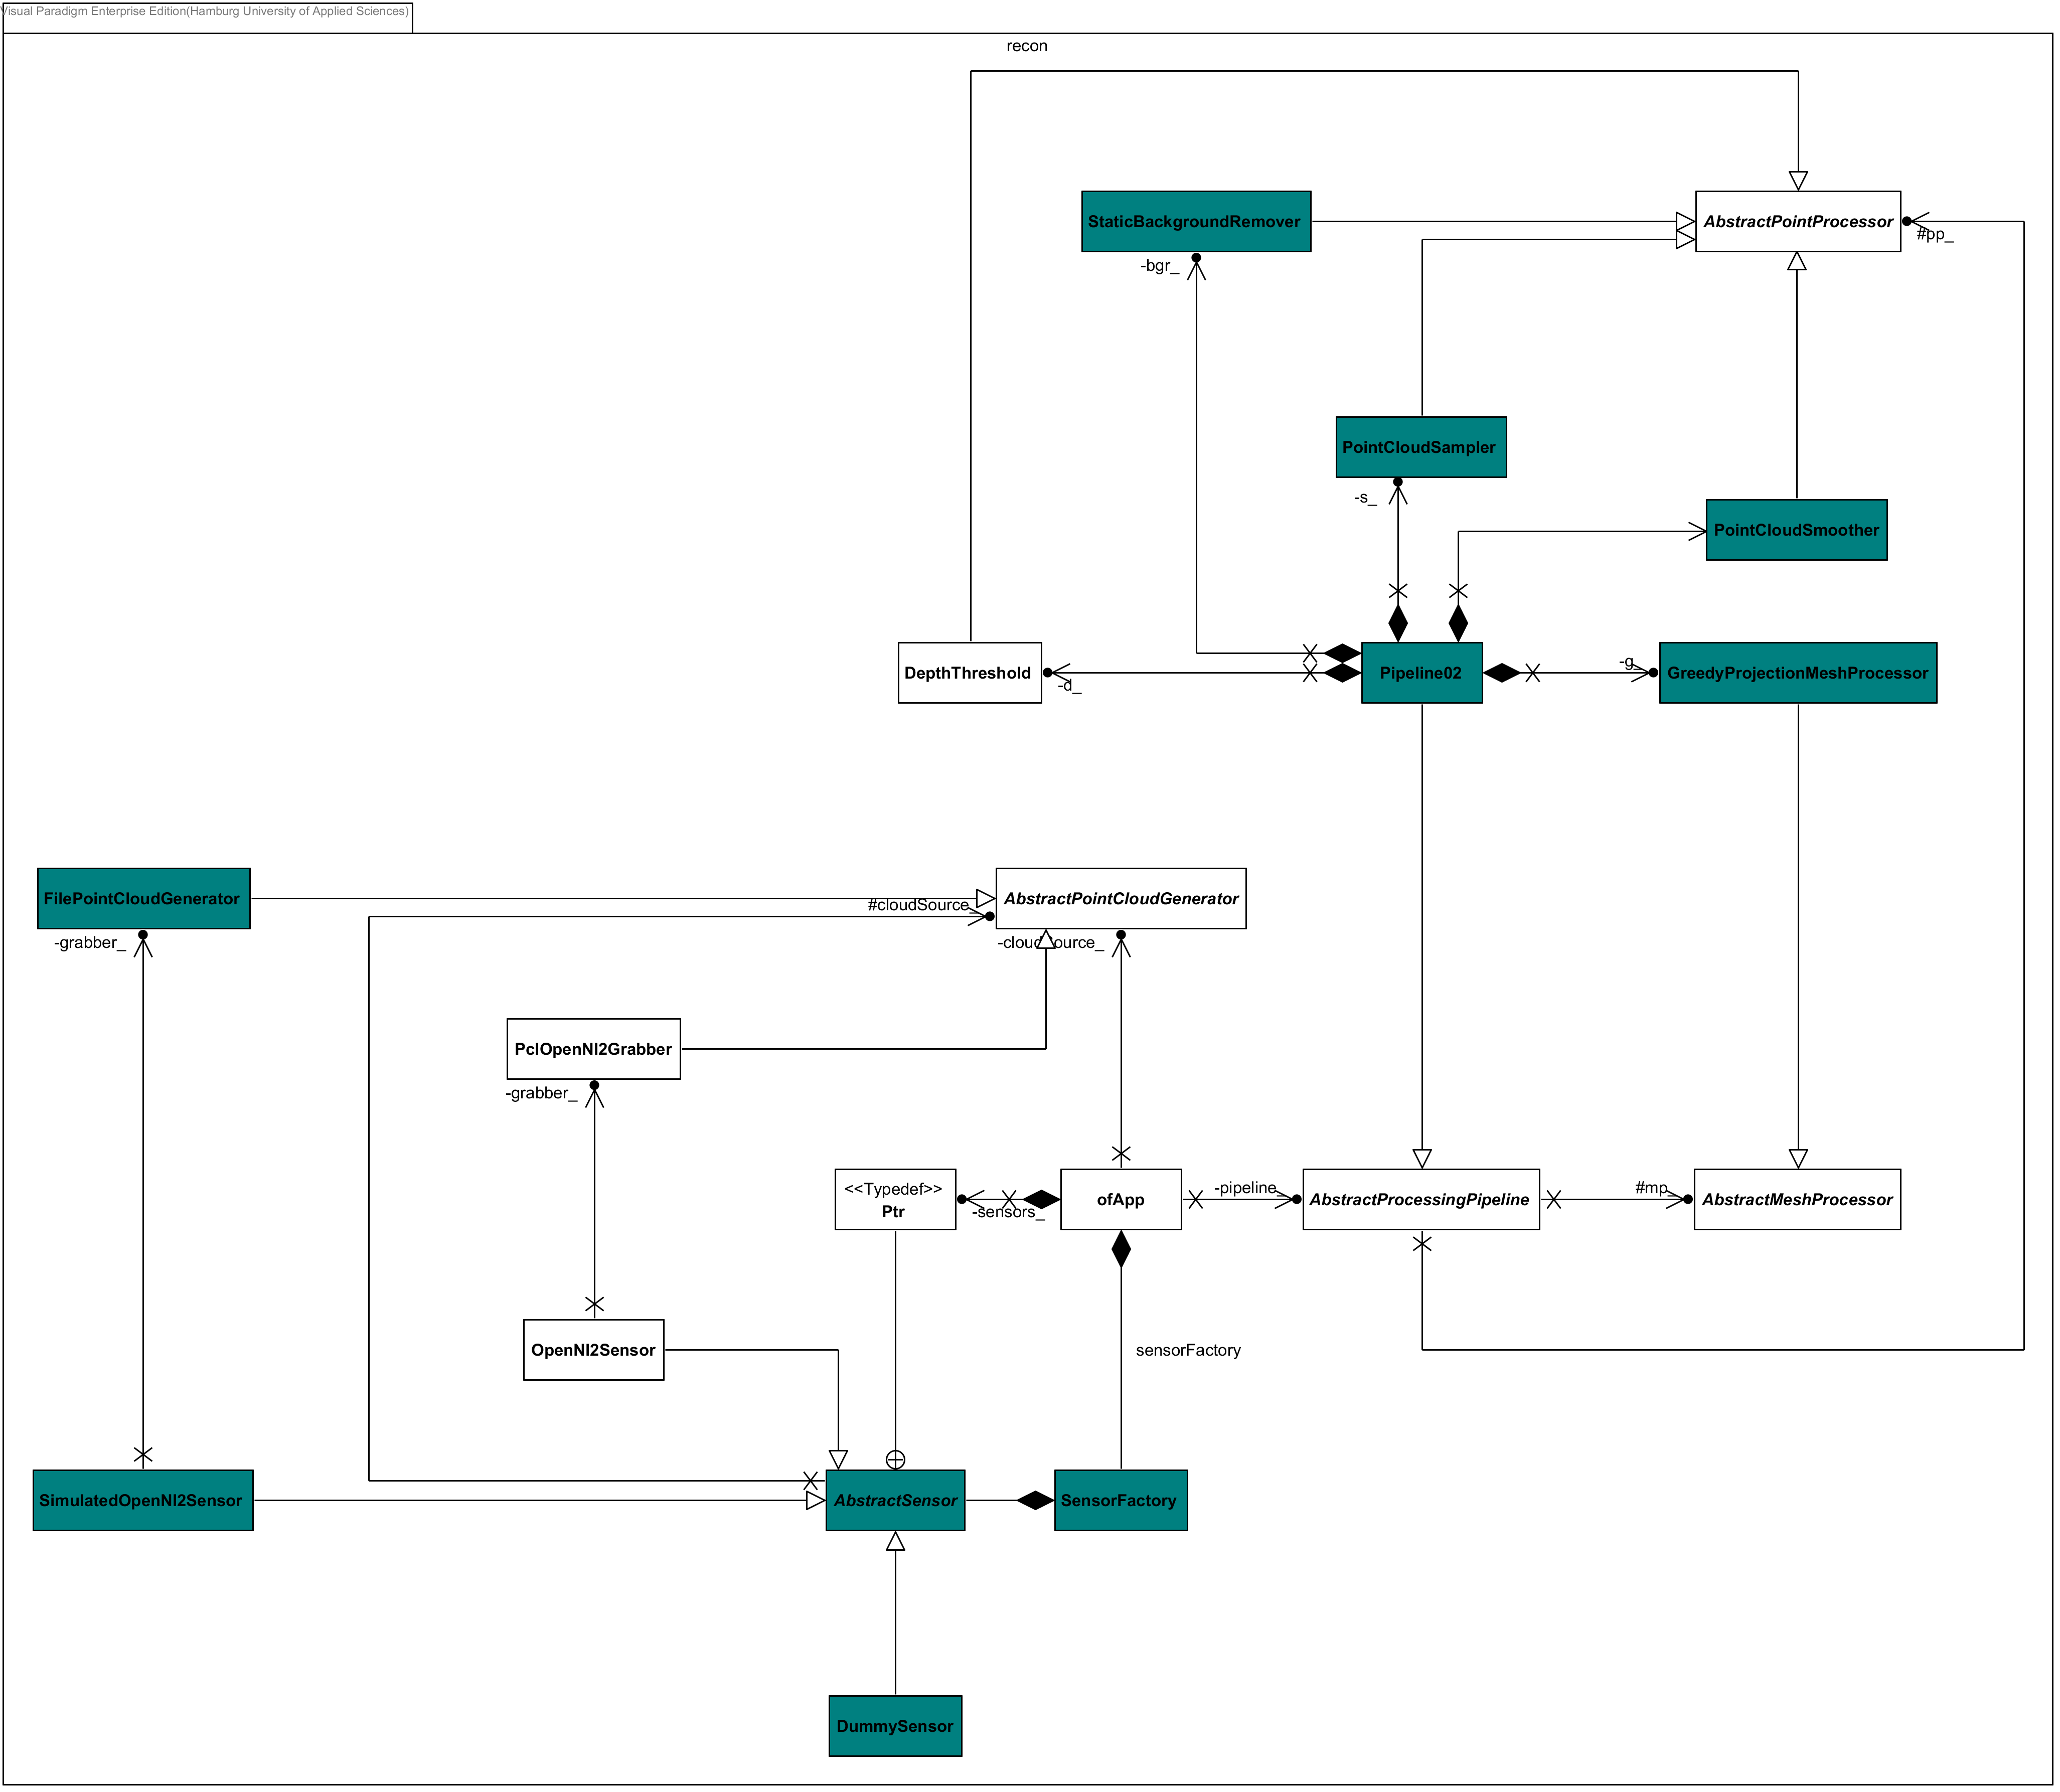
\includegraphics[width=\textwidth]{figs/class_diagram}
	\caption{Klassen Diagramm mit Erweiterung im Vergleich zu Projekt 1}
	\label{fig:classdiag}
\end{figure}


%Future work:
% Texturmapping durch Rückprojektion der Punkte auf Kameraebene.

\subsubsection{Nächste Schritte: } 
Zunächst gilt es die Punktwolkenvorverarbeitung zu 
vervollständigen um das Triangulationsergebnis zu optimieren. Anschließend ist 
eine Texturmappingkomponente zu entwicklen welche die nötigen Daten erzeugt um 
ein texturiertes 3D Modell rendern zu können. Auf dieser Basis kann dann eine 
Bewertung sowie Justierung des Rekonstruktionsergebnisses stattfinden. Als 
nächstes gilt es dann, das rekonstruierte Mesh an die Visualisierungskomponente 
des Projektsystems zu streamen, um die Wirksamkeit des Konzeptes in einer Mixed 
Reality Umgebung zu testen. Zu guter letzt wäre die Entwicklung einer komfortablen 
Kamerakalibrierungs-Lösung wünschenswert.

\section{Netzwerk-Middle C++ Implementierung}
Die C++ Implementierung der Netzwerk-Middleware ist in weiten Teilen abgeschlossen. 
Wie geplant wurde diese auf Basis der asynchronen Boost::asio Bibliothek für den 
Netzwerktransport entwickelt. Hierbei musste in größeren Teilen vom Konzept der C\# 
Referenzimplementierung abgewichen werden, da diese einige High-Level Konzepte 
verwendet, die so in C++ kaum umsetzbar sind. Ein essentieller Part der noch fehlt 
ist die Möglichkeit Callbacks für den Erhalt spezifischer Nachrichtentypen bei der 
Middleware zu registrieren. Aus Zeitgründen wurde diese Aufgabe zunächst hinten 
angestellt. Umfangreiche Tests zur Kommunikation mit den Implementierungen in C\# 
und Java stehen somit ebenfalls noch aus.

\section{Mesh-Streaming und Darstellung}
Zu diesem Teilthema ist noch keine praktische Arbeit vorgenommen worden. Einige Überlegungen zur Übertragung sowie Darstellung des rekonstruierten Modells sind dennoch angefallen.

Um das rekonstruierte Modell in einer 3D Umgebung darzustellen sind einige Daten 
erforderlich. Neben den eigentlichen Meshdaten, bestehend aus Vertizen inklusive 
Texturkoordinaten und Dreiecken als Triple von Punktindizes muss auch die 
kombinierte Textur bekannt sein. Ausserdem muss ein Ort im Welt-Koordinatensystem 
der 3D Umgebung festgelegt sein, welche die Basis der Vertizen des Meshes bestimmt.
Um eine Relation dieses Koordinatenursprungs zu einem Punkt in der Wirklichkeit zu 
erhalten, wäre der Einsatz eines markerbasierten Trackingverfahrens denkbar. Da sich 
in dem geplanten Setup sowohl die Kameras als auch der Koordinatenursprung nicht 
bewegen sollten, wäre diese Prozedur als Teil der Initialisierung des Systems zu 
realisieren. Somit bleiben die Mesh-Daten sowie die Textur, die Bild für Bild aufs 
neue benötigt werden. Die im Projekt entwickelte Netzwerk-Middleware hat sich im 
Rahmen der Anbindung des See-Through Displays bereits als tauglich erwiesen, Bilder 
in akzeptabler Auflösung und Framerate übertragen zu können. Dies bestätigt 
angfänglich naive Pläne, das Mesh-Streaming zunächst auf dieser Middleware zu 
versuchen. Da eine weitere Beschäftigung mit Kompressionsmöglichkeiten im Rahmen der 
Masterarbeit nicht mehr abzusehen ist, wird dieser Plan auch Bestand haben. Bei der 
Nachrichtendefinition für die Texturübertragung wird sich an der, für die 
Übertragung an das See-Through Display verwendeten, orientiert werden. Die 
Nachrichtendefinition für die Mesh-Daten besteht dann im Prinzip lediglich aus je 
einem Array für Vertizen, Texturkoordinaten und Punktindizes. Diese Nachrichten 
werden dann in einer noch zu entwickelnden Unity Komponente mit Hilfe des C\# 
Netzwerkadapters entgegengenommen, in eine für Unity geeignete Datenstruktur 
integriert und dargestellt.



\bibliographystyle{lnig}
\bibliography{literature}

\end{document}



